\documentclass{article}
\usepackage[french]{babel}
\usepackage{pdfpages}
% Set the citation style
\usepackage[
    backend=biber      % Specifies the backend to be used by BibLaTeX for processing the bibliography. 'biber' is the default backend.
]{biblatex}
\addbibresource{ref.bib} % Adds the bibliography resource file 'ref.bib' containing all the references.
\usepackage{hyperref}


\title{Candidature au prix de thèse de la Société Savante Francophone d'Apprentissage Machine}
\author{Hector Kohler}
\date{À Paris, le 21 Mars 2026}

\begin{document}

\maketitle
\noindent
Cher jury,\\

Vous trouverez dans ce document mon dossier de candidature complet pour le prix de thèse de la SSFAM 2026.
La plupart du document est en français avec certaines parties en anglais.
Par la présente candidature, je m'engage à présenter mes travaux lors de la Conférence sur l'Apprentissage automatique 2026 si je suis lauréat d'un prix.
\\

\noindent Merci par avance,\\
Respectueusement,\\
Hector Kohler
\tableofcontents{}
\newpage
\section{Curriculum Vitae}
Mon manuscrit de thèse est disponible à cette adresse en attendant sa publication sur HAL: \url{https://github.com/KohlerHECTOR/thesis/blob/main/these.pdf}
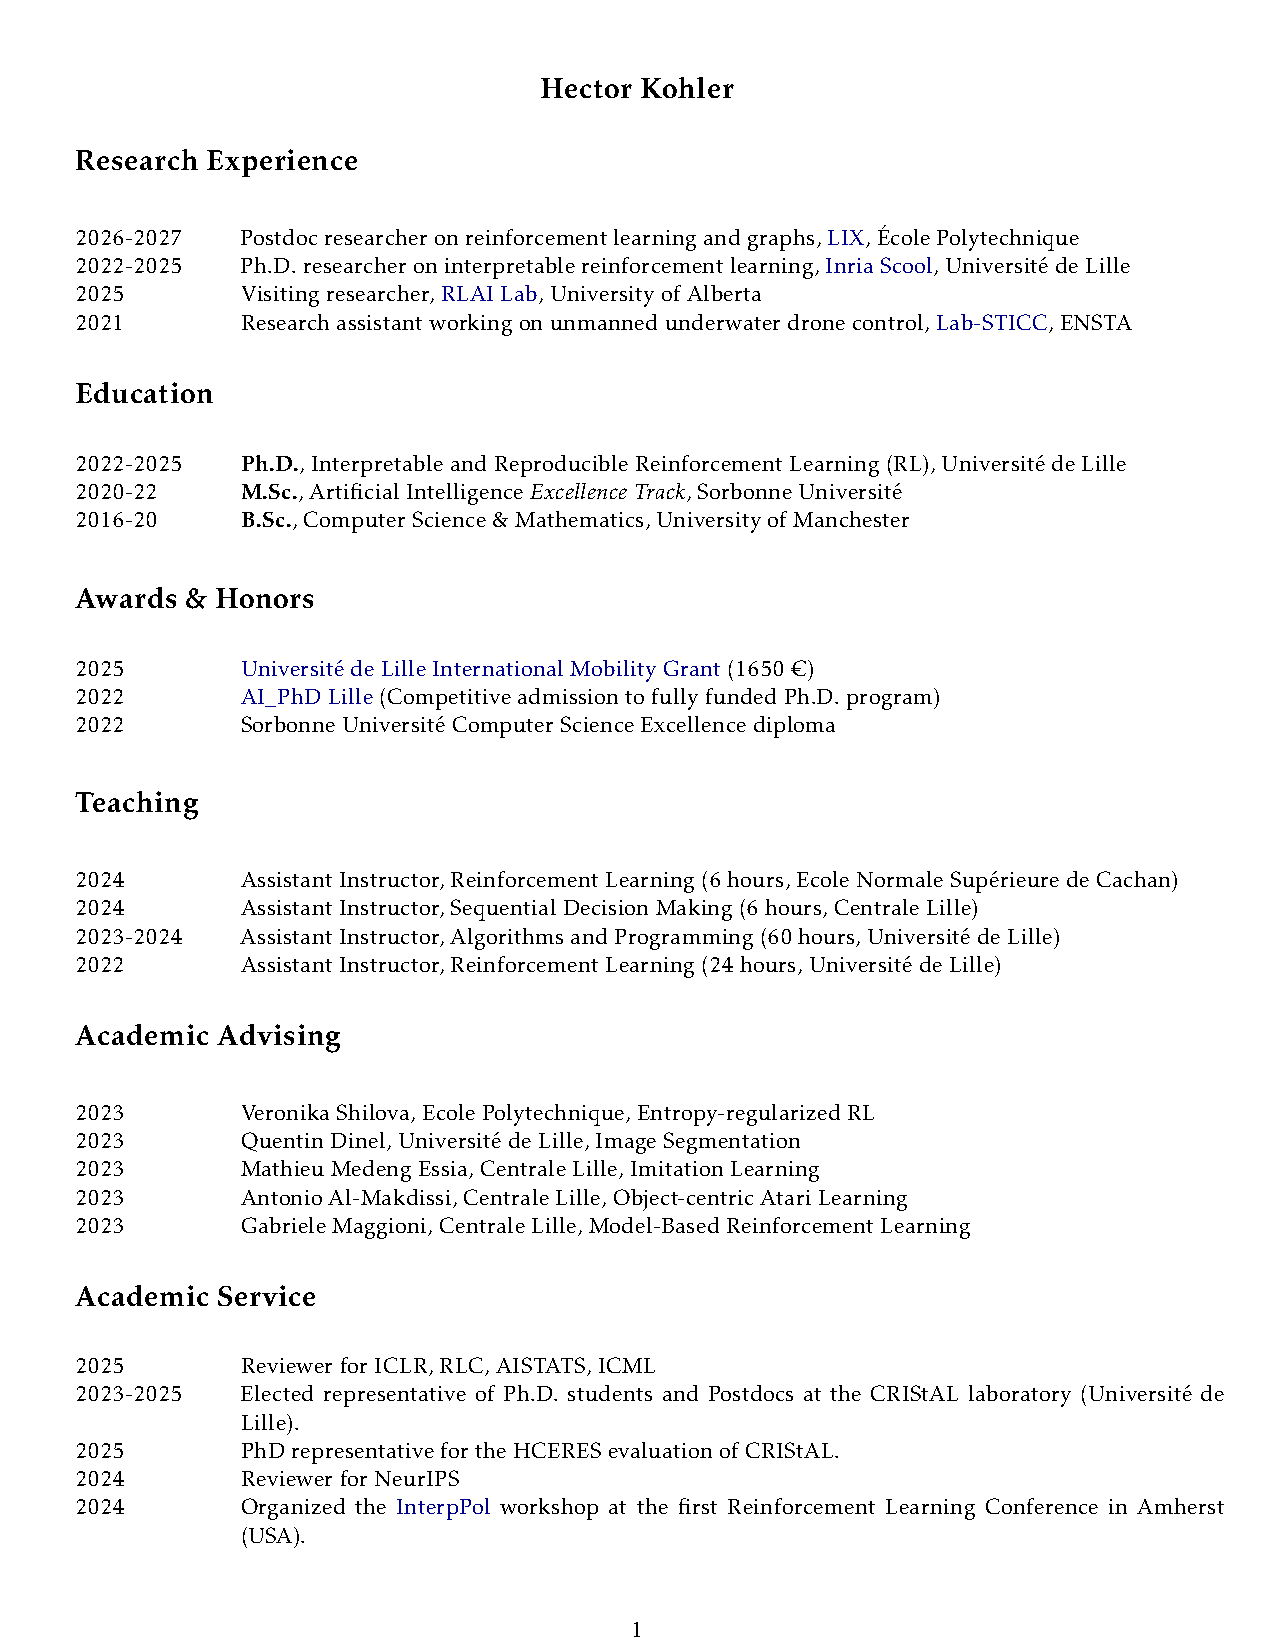
\includepdf[pages={-}]{cv.pdf}
\newpage
\section{Résumé de la thèse}
Dans cette thèse, nous abordons le problème de la prise de décision séquen-\\tielle interprétable.
Nous étudions l'interprétabilité à travers le prisme des classes de modèles utilisées comme politiques pour les processus de décision markoviens (PDM) ou comme prédicteurs pour les tâches de classification, avec un accent particulier sur les arbres de décision, souvent considérés comme plus interprétables que les réseaux neuronaux.
Les arbres de décision sont interprétables car les humains peuvent lire les opérations de l'arbre depuis la racine jusqu'aux feuilles, ce qui en fait le modèle de référence lorsque la vérification humaine est requise, comme dans les applications médicales.
Cependant, les arbres de décision ne sont pas dérivables, ce qui les rend difficiles à optimiser, contrairement aux réseaux neuronaux entraînés efficacement par descente de gradient.
Les approches existantes d'apprentissage par renforcement interprétable apprennent généralement des arbres souples (non interprétables en l'état) ou procèdent de manière indirecte (entraîner un réseau neuronal puis distiller un arbre pour l'imiter), sans garantie d'optimalité pour le problème initial.
Le manuscrit est organisé en trois parties, chacune apportant une contribution distincte.

La première partie vise à apprendre directement des politiques d'arbres de décision pour un PDM par apprentissage par renforcement.
Nous commençons par une étude de reproductibilité des algorithmes existants qui optimisent un compromis entre interprétabilité et performance dans un PDM augmenté.
Nous concluons que les algorithmes d'apprentissage par imitation, bien qu'ils n'optimisent pas directement les performances sur la tâche en aval, produisent de meilleures politiques d'arbres de décision avec un nombre similaire de nœuds internes.
Afin de comprendre cet échec, nous montrons que l'apprentissage direct de politiques d'arbres de décision par renforcement se reformule comme un problème d'optimisation dans un processus de décision markovien partiellement observable (PDMPO).
Grâce à une expérimentation approfondie dans un environnement très contrôlé, nous identifions l'observabilité partielle comme le principal mode de défaillance de cette approche directe.
Pour corroborer cette conclusion, nous montrons que lorsque les observations contiennent toute l'information sur l'état caché --- c'est-à-dire quand le PDMPO devient complètement observable --- les algorithmes d'apprentissage par renforcement convergent vers les politiques d'arbres de décision optimales.
Ce parallèle entre l'apprentissage des arbres de décision et la résolution des PDMPOs explique pourquoi, en pratique, il est souvent plus facile de distiller un réseau neuronal expert en arbre que d'apprendre l'arbre de décision à partir de zéro.
Un article regroupant les résultats de cette première partie a été soumis à la conférence RLC 2026~\cite{pomdp}.

De manière surprenante, la classe de PDMPOs faciles à résoudre identifiée dans la première partie --- ceux où les observations sont suffisamment informatives --- comprend les problèmes d'apprentissage supervisé.
Ce fait conduit à la conception d'un nouvel algorithme d'induction d'arbres de décision dans la deuxième partie du manuscrit.
Nous formulons l'induction d'arbres de décision comme la résolution d'un PDM où les états sont des exemples d'apprentissage et les actions sont des nœuds candidats d'arbres de décision.
Nous introduisons les arbres de décision par programmation dynamique (DPDT), une classe d'algorithme qui choisit adaptativement les actions à l'aide d'heuristiques gloutonnes, puis résout le PDM par programmation dynamique.
Des évaluations et comparaisons approfondies montrent que DPDT calcule des arbres de décision quasi-optimaux en une fraction du temps requis par les solveurs optimaux existants.
De plus, DPDT est compétitif dans de nombreuses applications d'apprentissage automatique~: ses capacités de généralisation --- en arbres uniques comme en ensembles --- sont à la pointe de la technologie par rapport aux algorithmes gloutons et optimaux.
Bien que cette partie puisse sembler orthogonale aux deux autres, car l'accent est mis sur les performances plutôt que sur l'interprétabilité, elle démontre que l'interprétabilité peut être un levier de performance et pas seulement une contrainte de transparence.
Les résultats de cette deuxième partie ont été publiés à la conférence KDD 2025~\cite{dpdt}, et nous avons développé \texttt{DPDT}\footnote{\url{https://github.com/KohlerHECTOR/DPDTreeEstimator}}, un estimateur compatible avec \texttt{scikit-learn} qui implémente cet algorithme.
Dans la figure~\ref{fig1}, nous montrons les performances de DPDT par rapport à d'autres algorithmes de pointe pour la classfication.

Les deux parties précédentes reposent sur l'hypothèse que les arbres de décision sont un modèle interprétable. Mais est-ce vraiment le cas~?
Dans la troisième et dernière partie, nous nous attaquons à des questions plus générales~: peut-on mesurer l'interprétabilité sans intervention humaine~? Les arbres de décision sont-ils réellement plus interprétables que les réseaux neuronaux~?
Nous proposons de mesurer l'interprétabilité d'un modèle à l'aide de la vitesse d'infé-\\rence et de la taille en mémoire, deux métriques qui font écho à la notion de simulabilité reliant l'interprétabilité à la complexité computationnelle classique.
Nous montrons que pour que ces mesures aient un sens lors de la comparaison de modèles issus de différentes classes, il est nécessaire de déployer les modèles dans un langage commun comme Python.
Après avoir séquencé toutes les opérations au sein d'un modèle et les avoir exécutées sur le même matériel, nous obtenons des mesures d'interprétabilité comparables qui concordent avec les résultats obtenus par des études utilisateurs.
Enfin, nous montrons qu'il n'existe aucune classe de modèles offrant un meilleur compromis interprétabilité-performance pour l'ensemble des tâches.
Ce résultat souligne la nécessité d'une méthodologie rigoureuse en recherche sur l'interprétabilité~: il ne suffit pas de se fier à l'hypothèse selon laquelle les réseaux neuronaux sont moins interprétables que les arbres de décision.
Les résultats préliminaires de cette partie ont été présentés au 17th European Workshop on Reinforcement Learning~\cite{interpreter} et au Workshop on Programmatic Reinforcement Learning~\cite{eval}.
Les expériences de cette partie s'appuient sur \texttt{Interpretable RL Zoo}\footnote{\url{https://github.com/KohlerHECTOR/interpretable-rl-zoo}}, une librairie de politiques interprétables écrites en Python pure pour différents environnements \texttt{gymnasium}.
Dans la figure~\ref{fig2}, nous montrons le compromis performances-interprétabilité de différentes classes de politiques de décision.

\begin{figure}
    \centering
    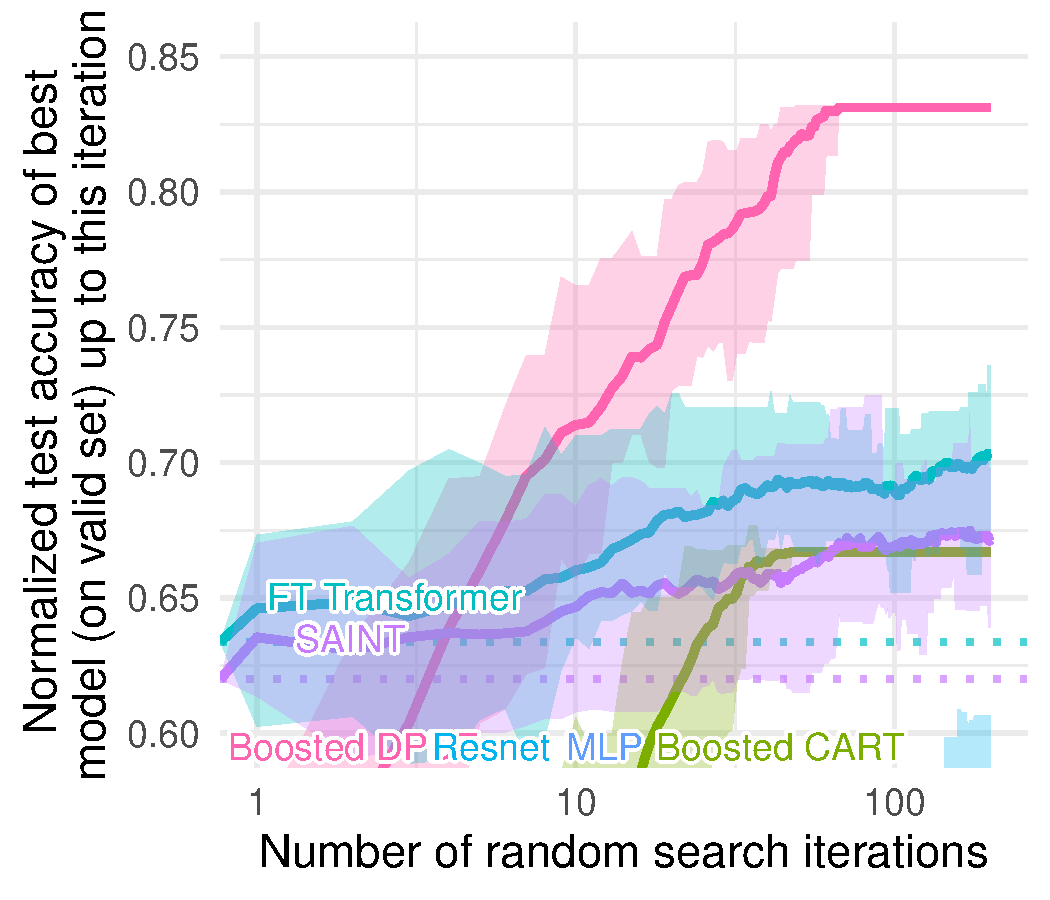
\includegraphics[width=0.5\textwidth]{random_search_classif_numerical_boosting_all_notgb.pdf}
    \caption{Précisions normalisées de différents classifieurs sur des données tests nouvelles. Les performances sont aggrégées pour 16 tâches de classification difficiles. On observe en rose que les performances de notre classifieurs Boosted DPDT sont supérieures à celles des autres modèles apres quelques itérations de recherche d'hyperparamètres.}\label{fig1}
\end{figure}


\begin{figure}
    \centering
    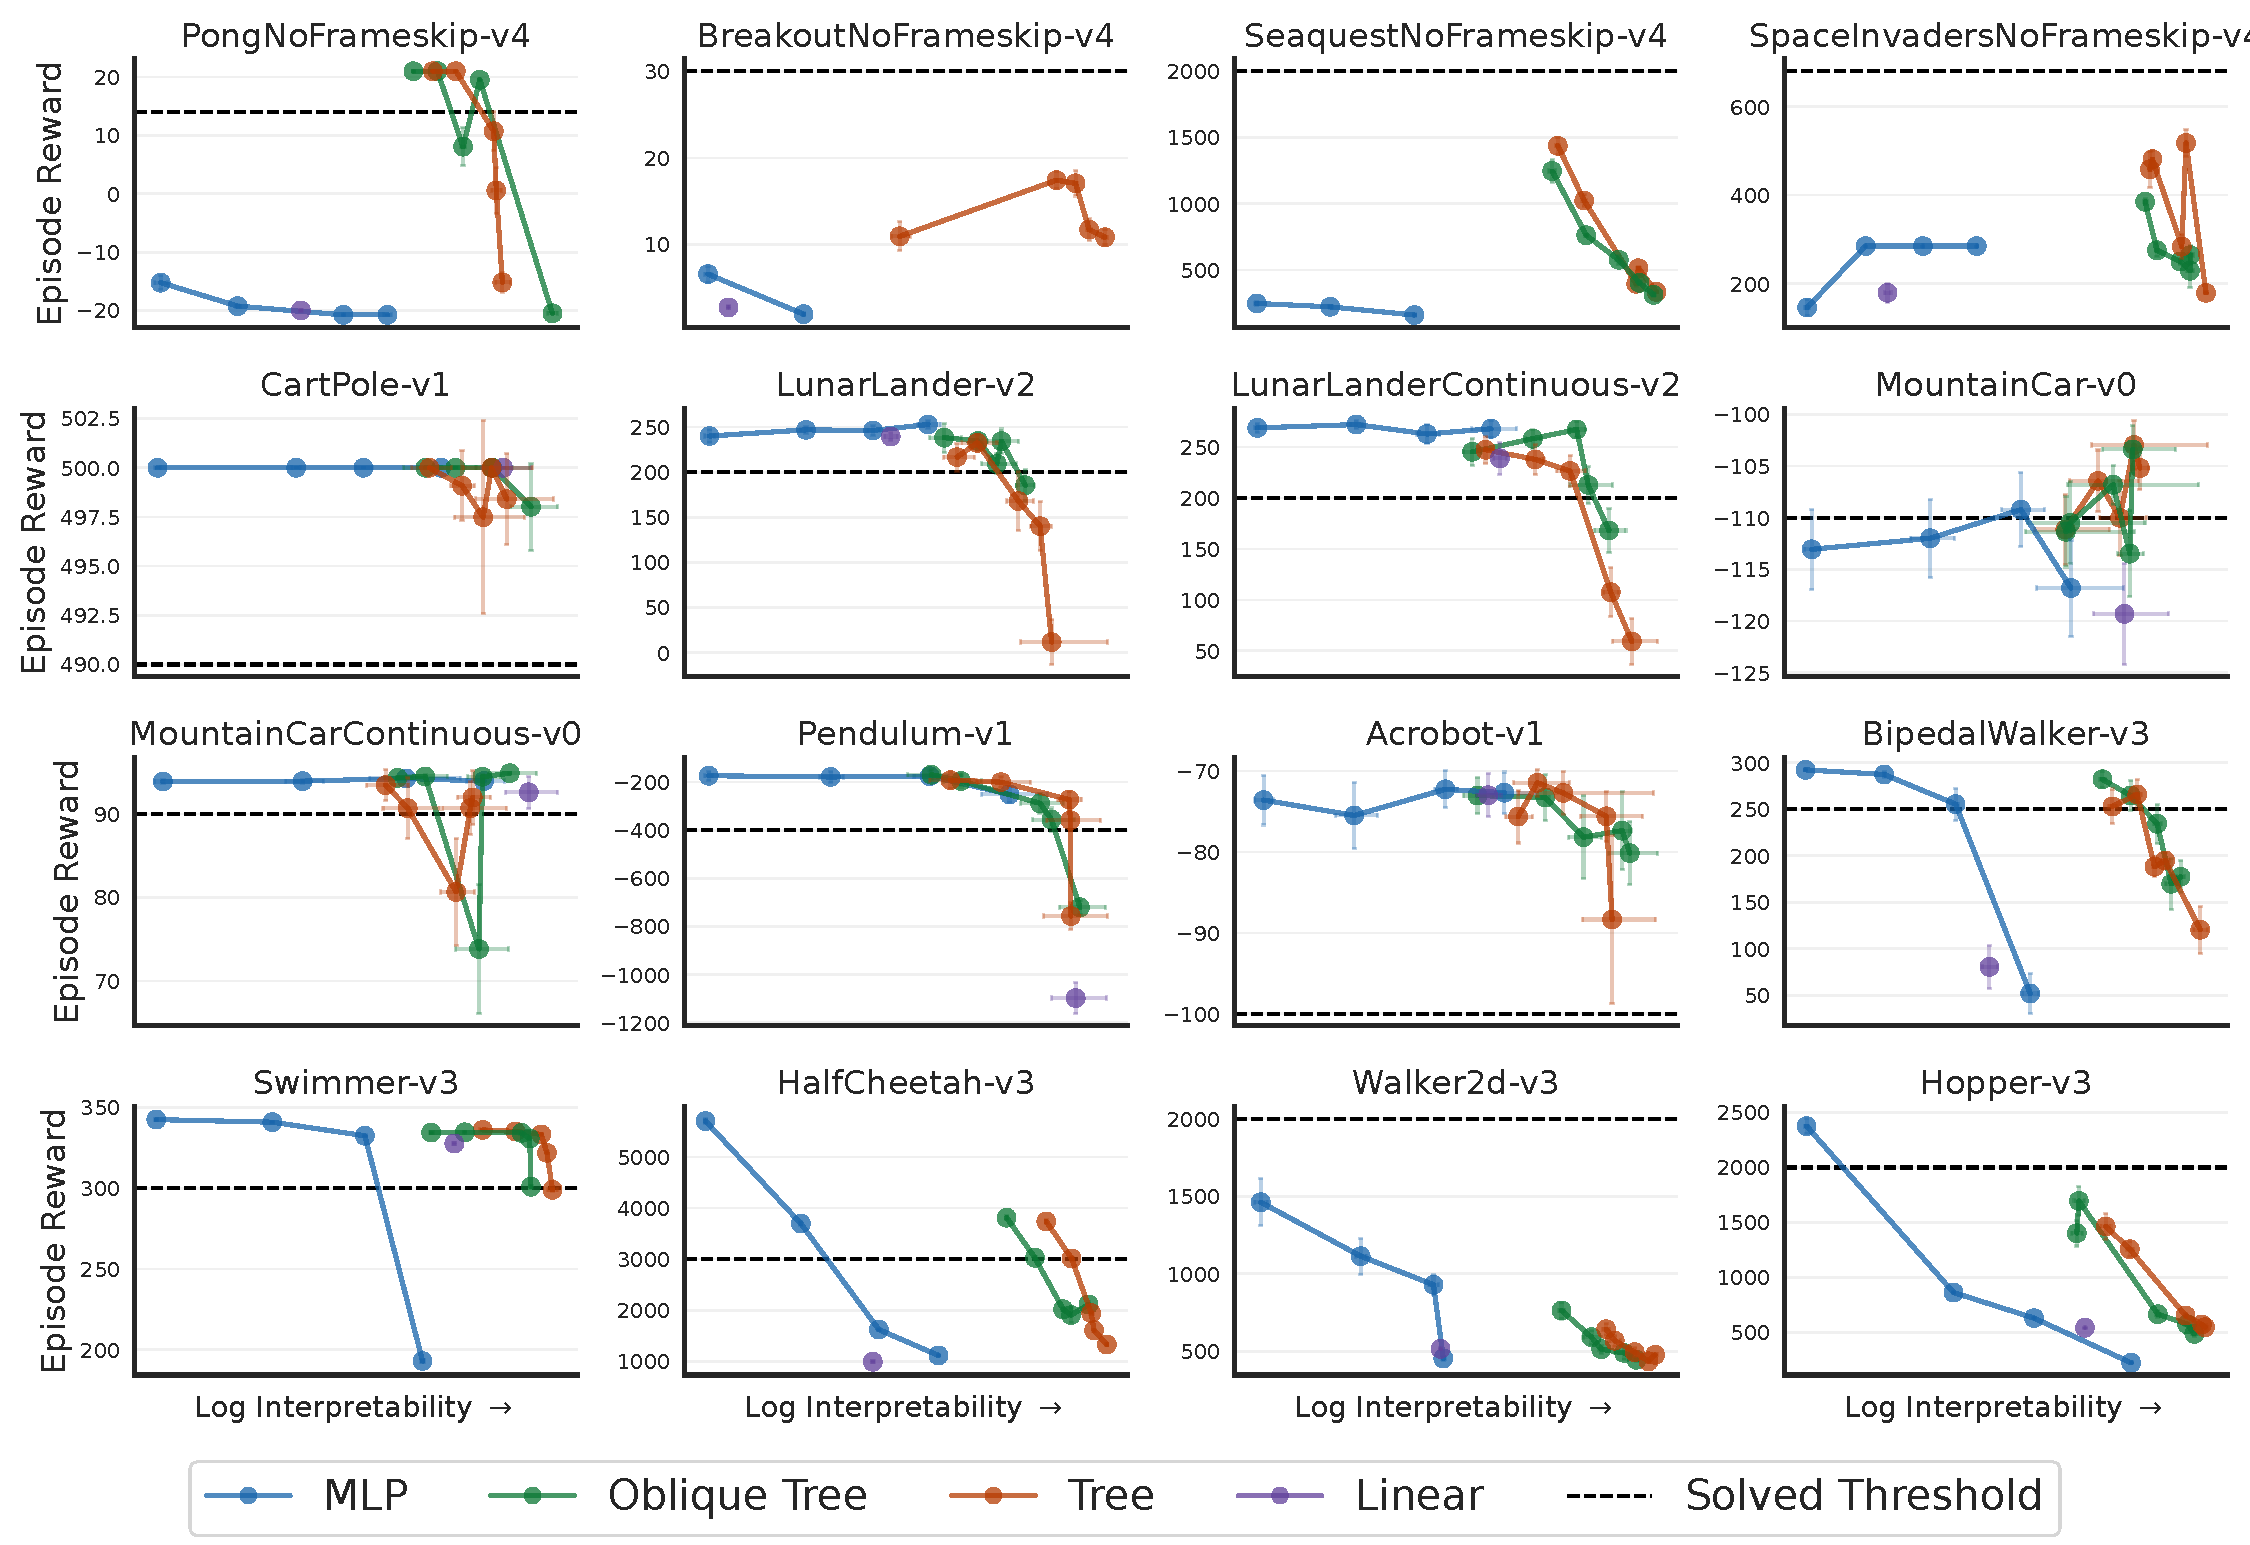
\includegraphics[width=0.9\textwidth]{trade_off.pdf}
    \caption{Compromis performances-interprétabilité de différentes classes de politiques de décision pour différents PDMs standards. On peut voir qu'il n'éxiste aucune classe de politique qui domine les autres sur tous les PDMs testés. Par exemple, sur Swimmer, ce sont les arbres de décision qui ont le meilleur compromis performances-interprétabilité, tandis que sur la version continue du MountainCar, ce sont les politiques linéaires.}\label{fig2}
\end{figure}

\printbibliography{}
\newpage
\section{Rapports de pré-soutenance et rapport de soutenance}
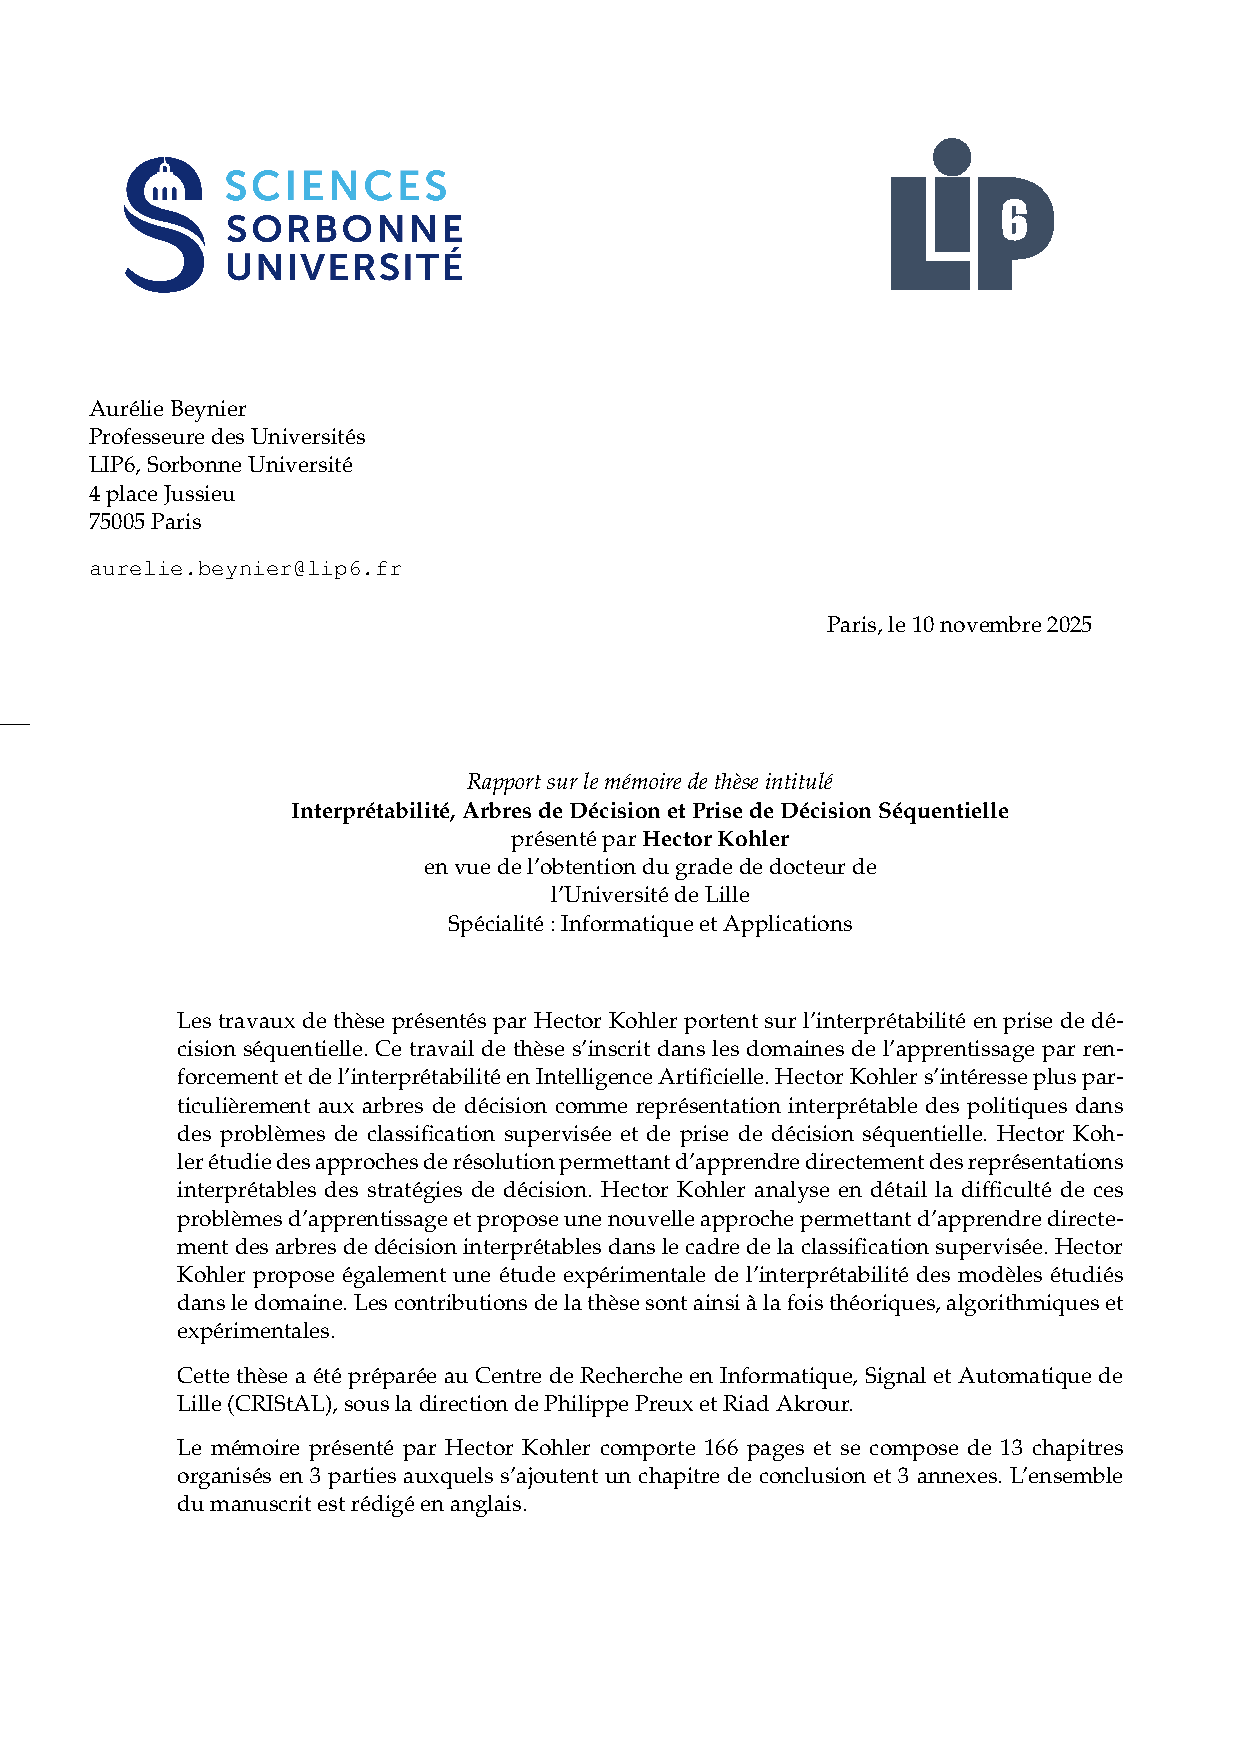
\includepdf[pages={-}]{rapport_beynier.pdf}
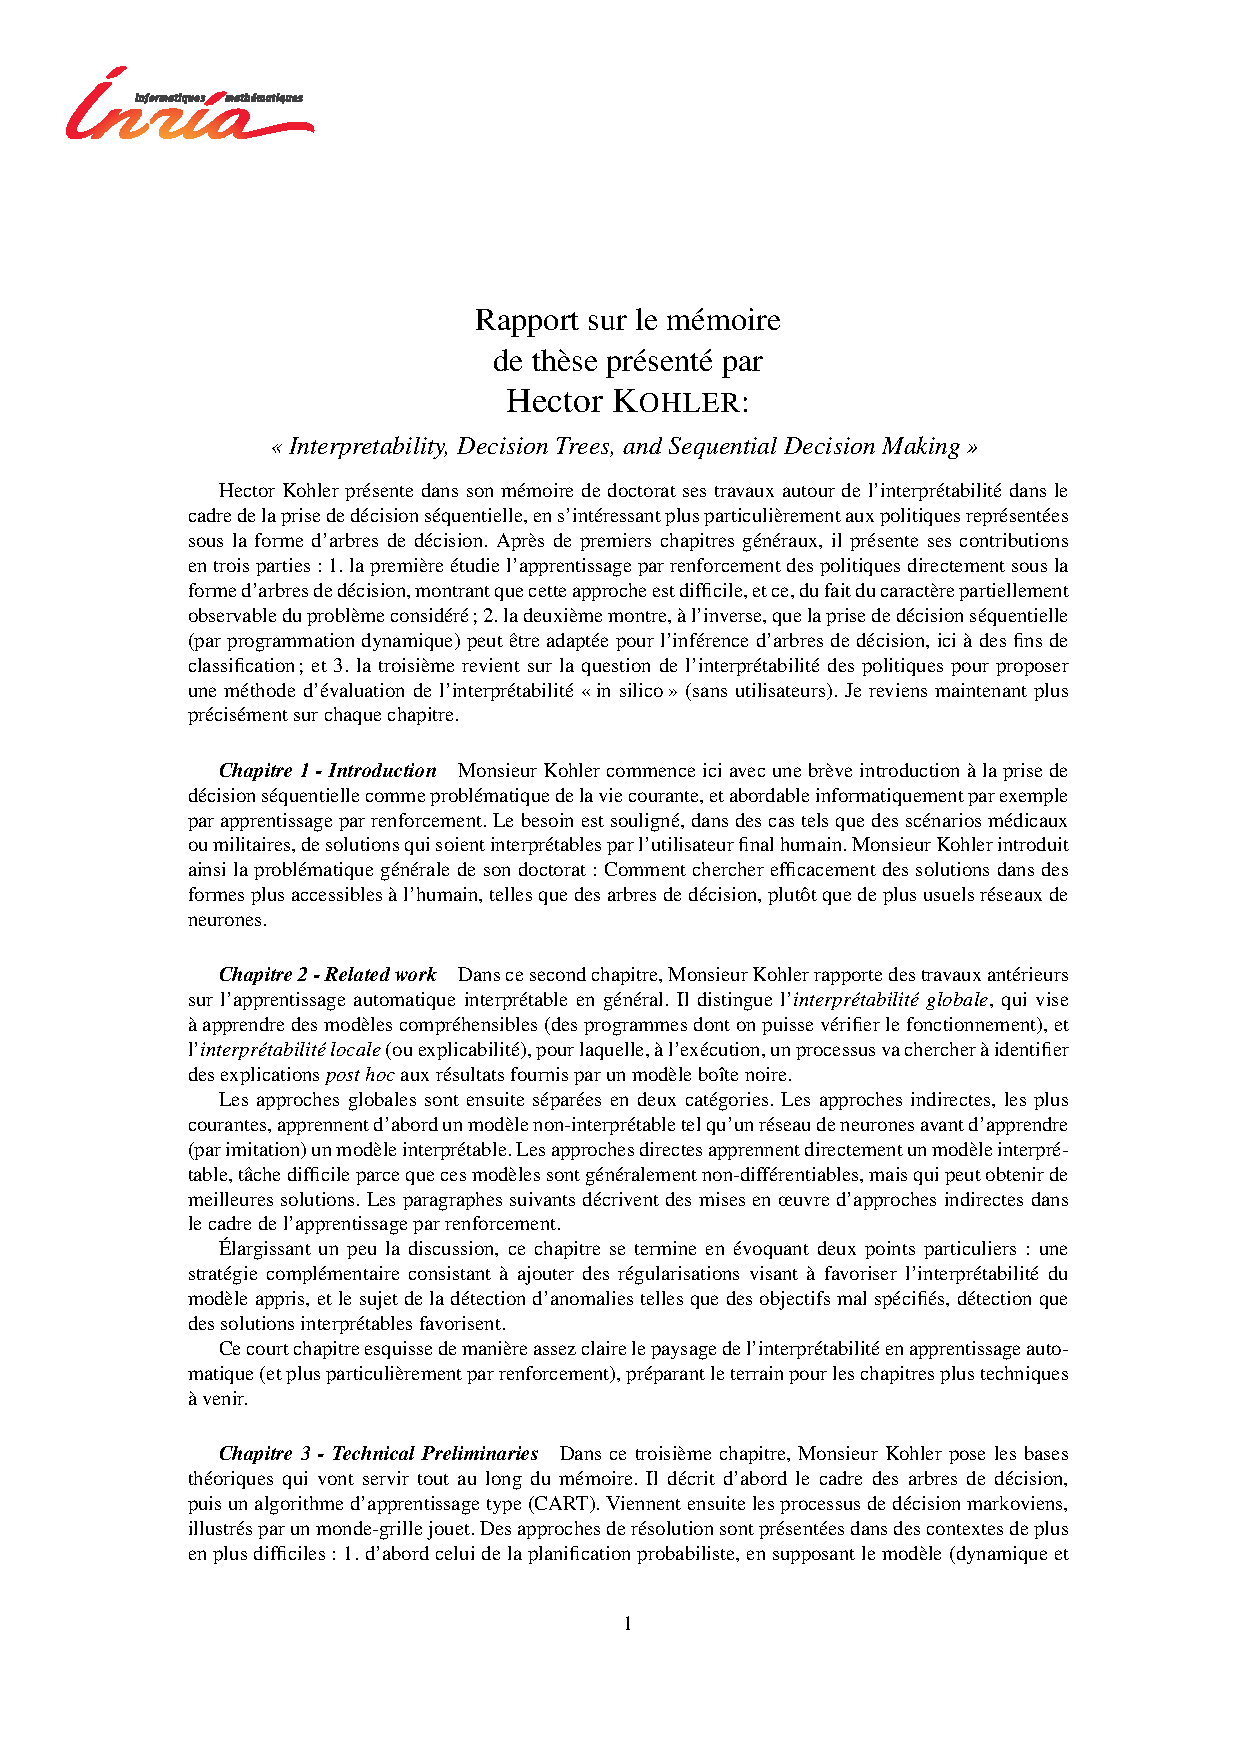
\includepdf[pages={-}]{rapport_buffet.pdf}
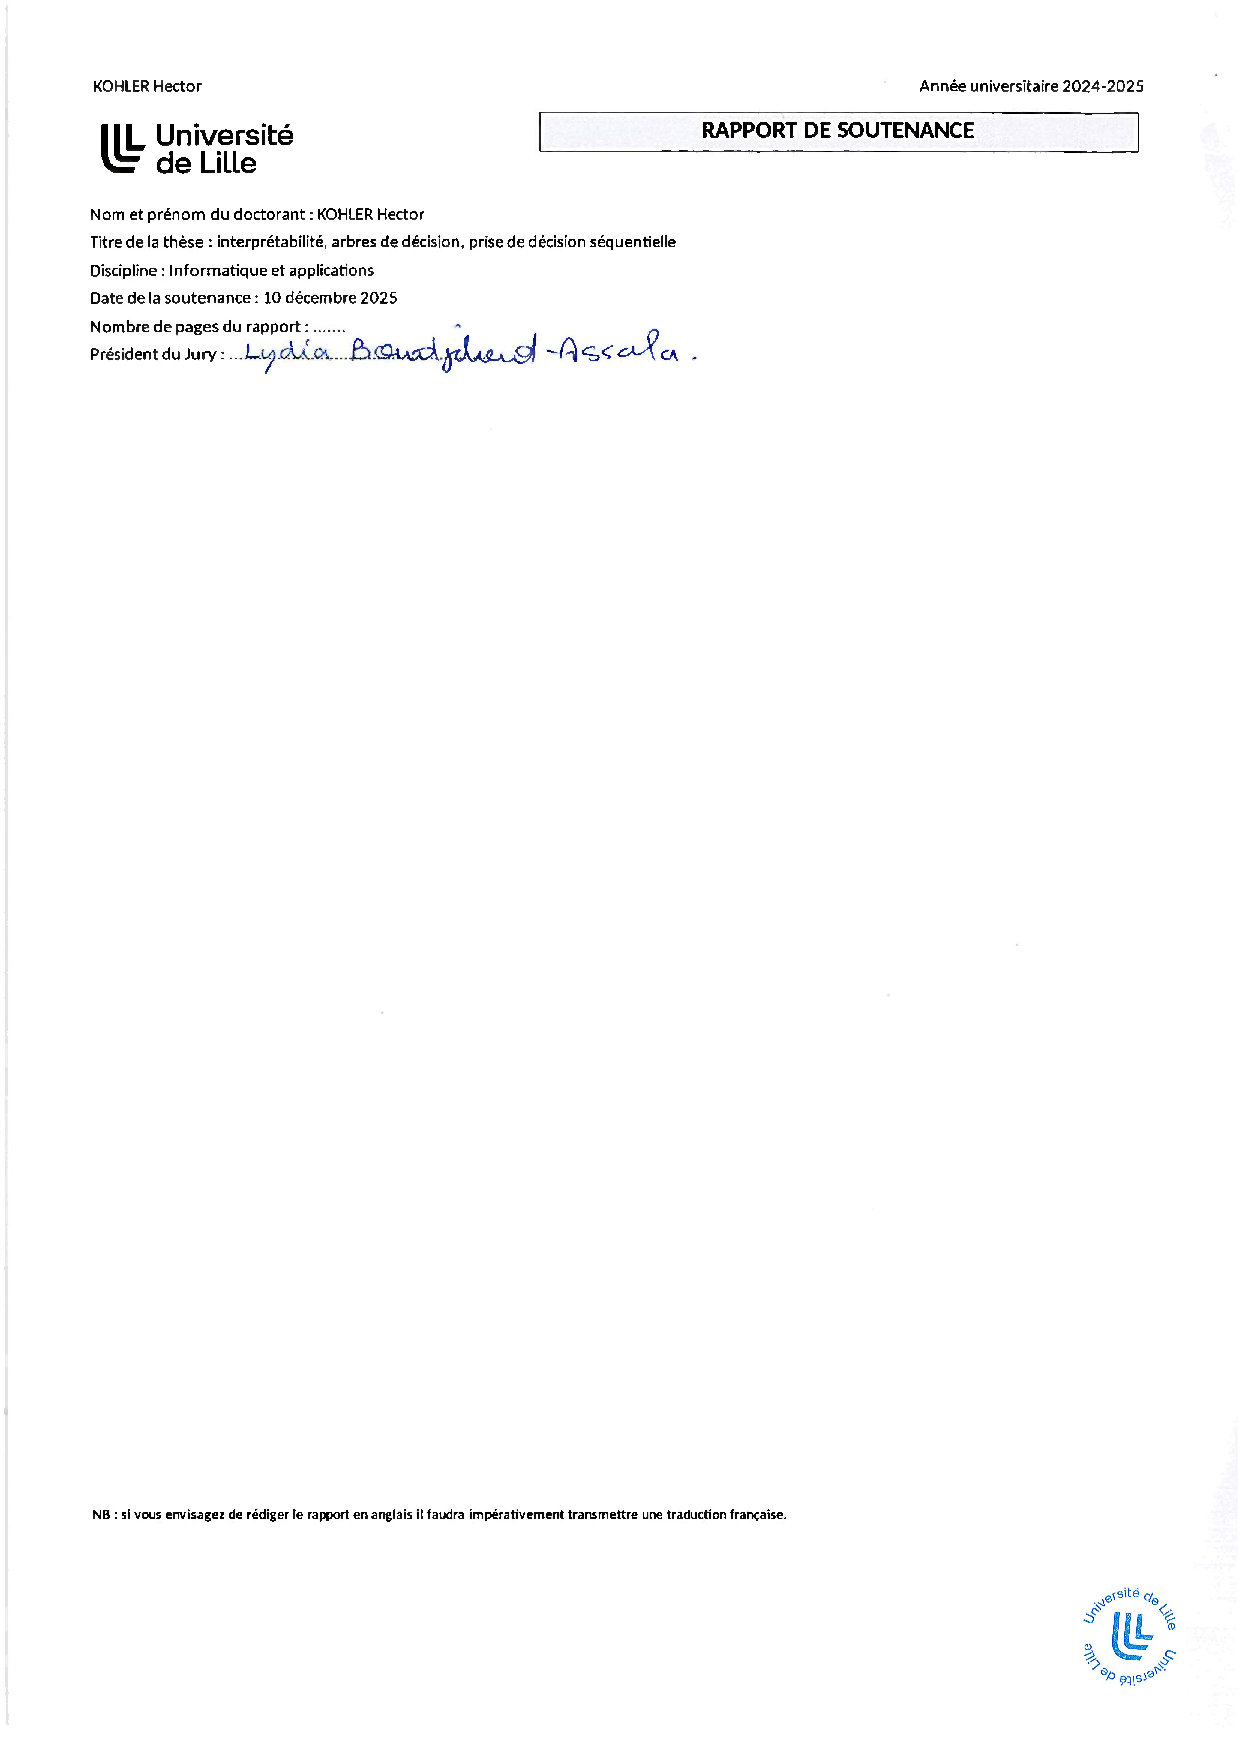
\includepdf[pages={-}]{rapport_soutenance.pdf}
\newpage
\section{Lettre de soutien de la direction de thèse}
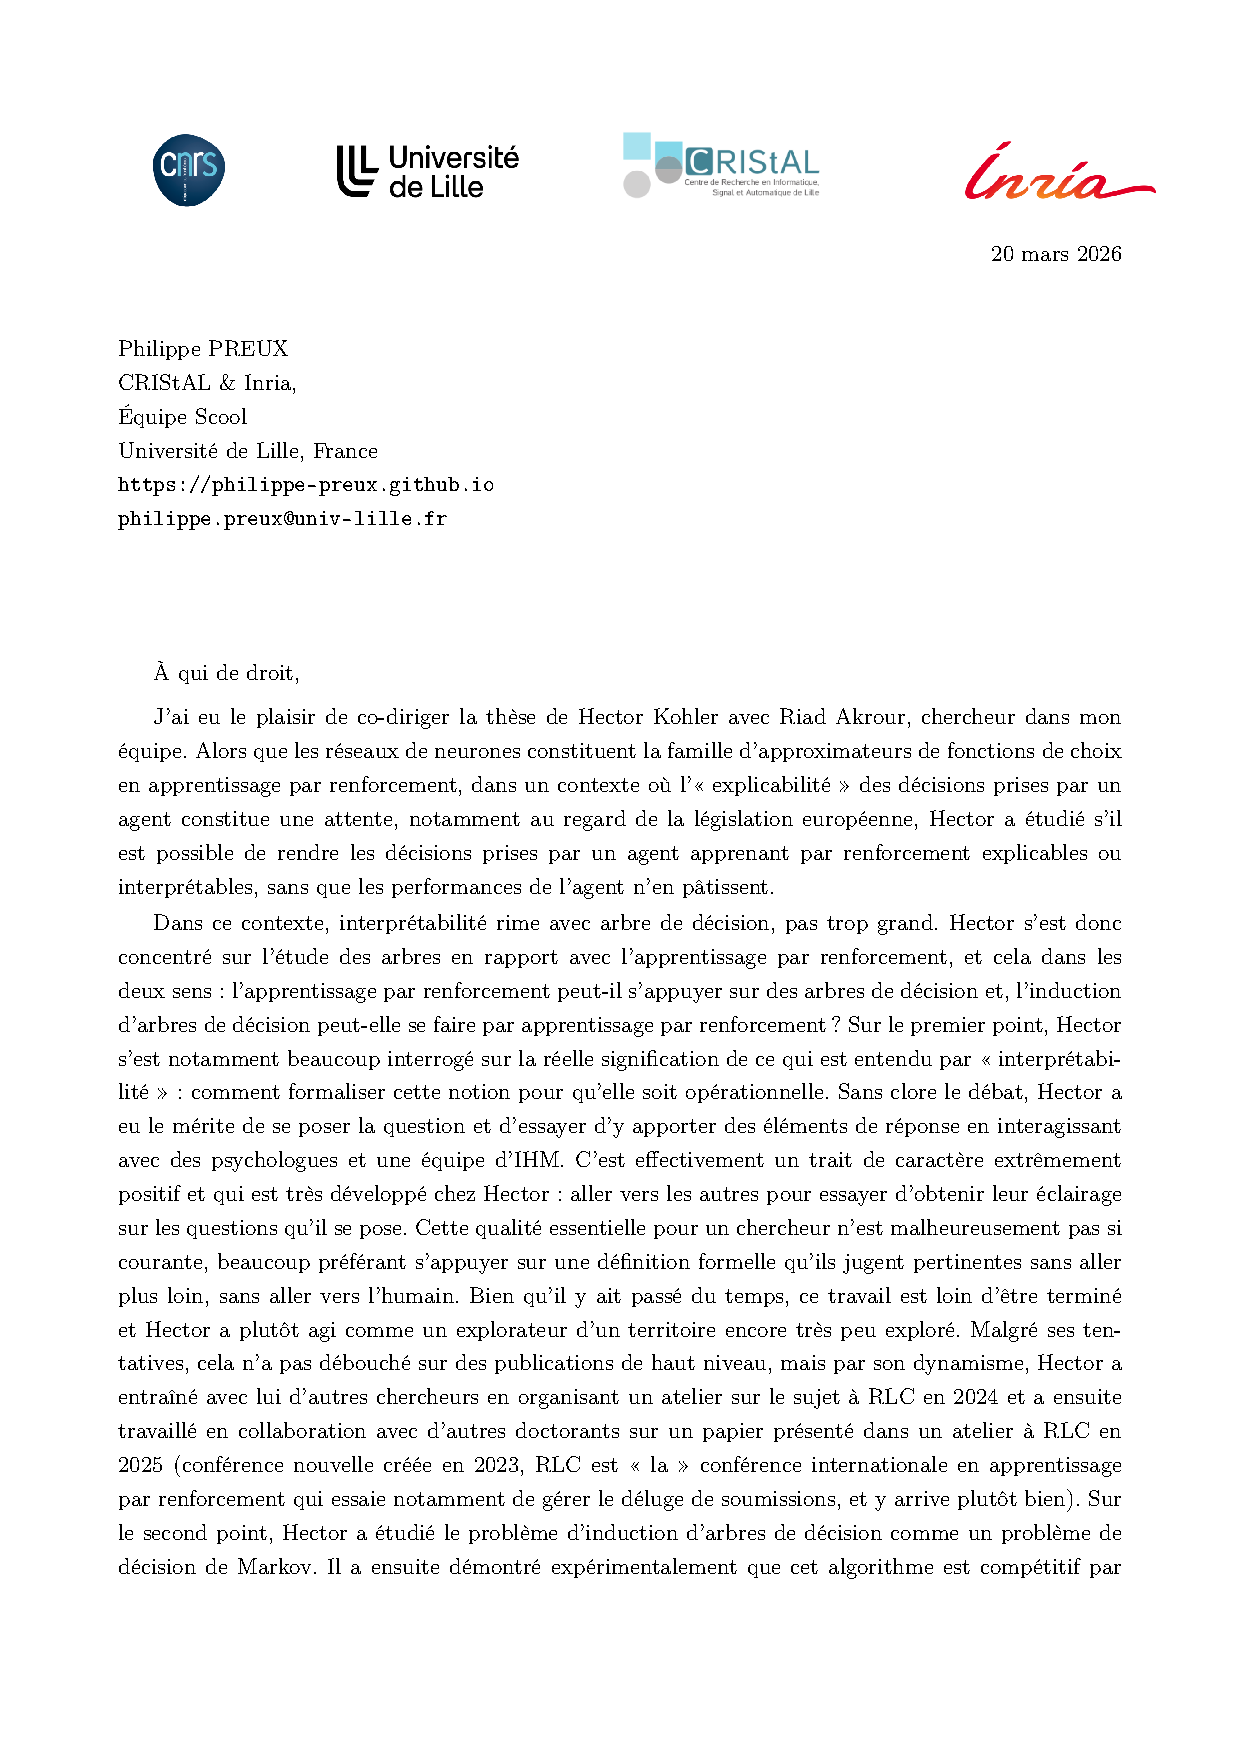
\includepdf[pages={-}]{hector.ssfam.pdf}
Merci
\end{document}